
\section{Algorithm Implementation}\label{sec:algo-impl}


\subsection{Multi-Trajectories Collection}

\begin{figure}[h]
\centering
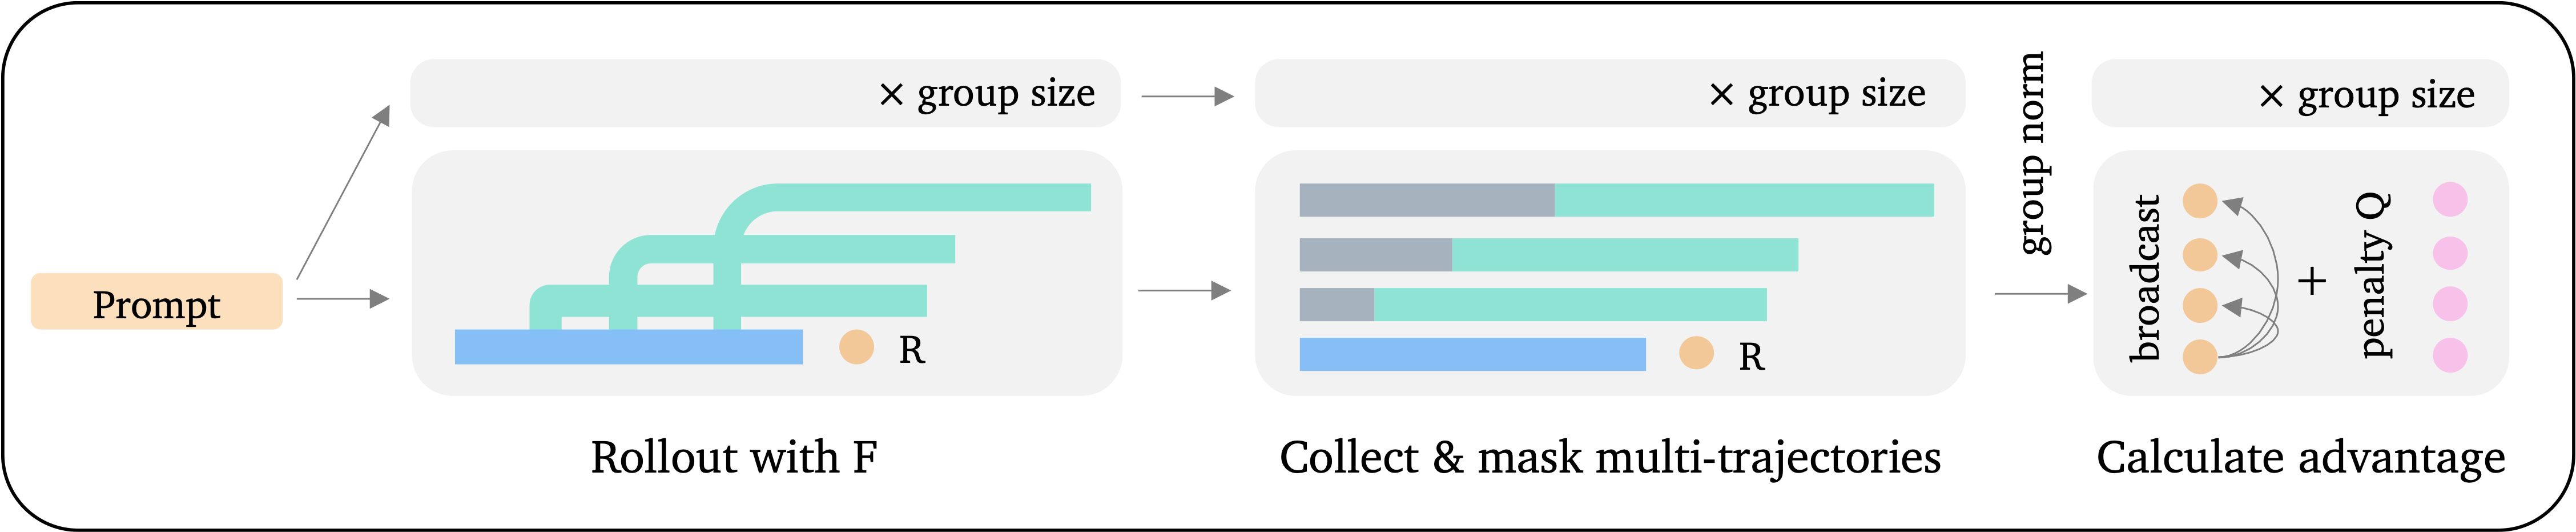
\includegraphics[width=1\columnwidth]{figs/multitraj.png}
\end{figure}

For practical implementation of model training, instead of concatenating all sub-trajectories into one sequence, we keep them as separate causally conditioned sequences, as shown above. Therefore, training with context folding is not directly compatible with existing training infrastructures (e.g., in Verl).


\subsection{Asynchronous Long-Horizon Agent Rollout}\label{sec:async-rollout}

\begin{figure}[h]
\centering
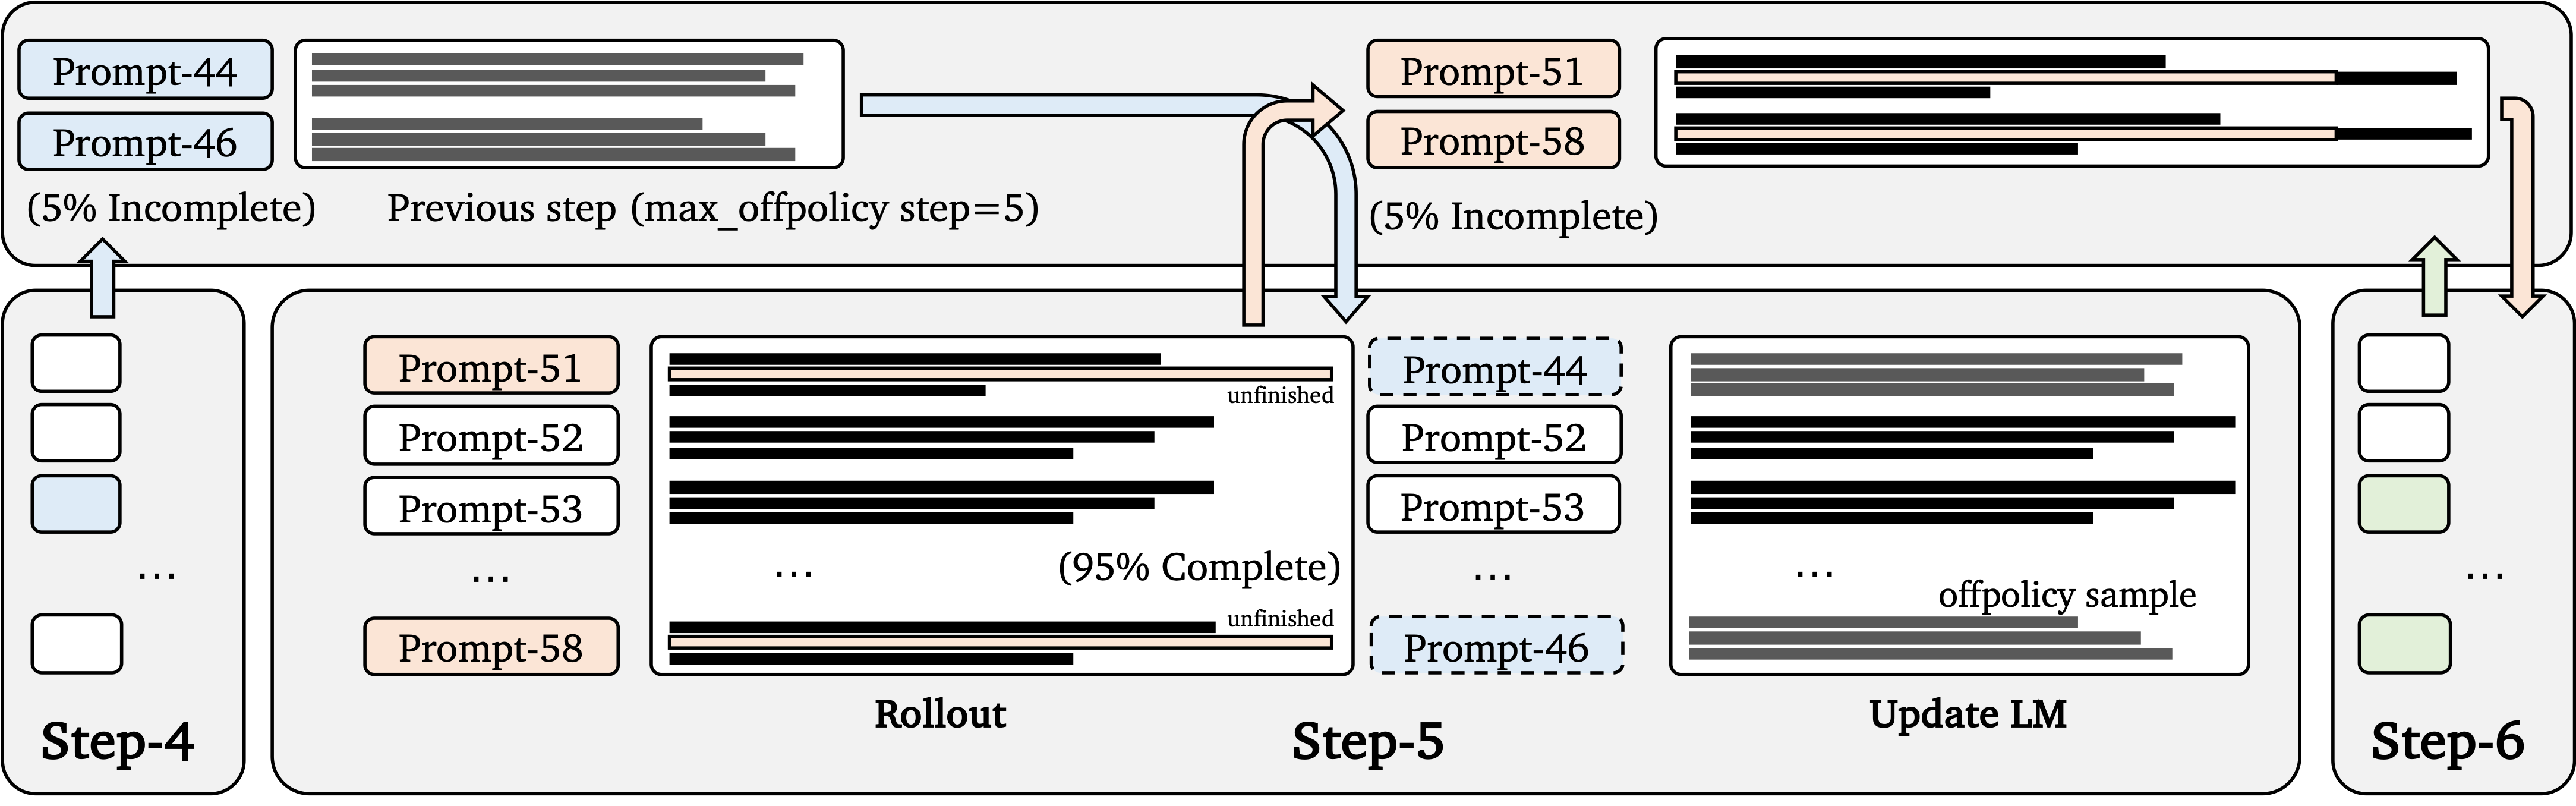
\includegraphics[width=1\columnwidth]{figs/async.png}
\end{figure}

The rollout time of long-horizon agents is imbalanced, which causes a “bubble” in computation, where faster jobs wait for the longest one to finish. In our training setup, we mitigate this by adding an additional standalone rollout process: the main rollout process stops once it completes 95\% of the prompts (this hyperparameter is adjusted based on the GPU configuration), and the remaining jobs are handled by the standalone process. The data used for updating the LM include both (i) the 95\% of the current batch and (ii) the prompts from the previous step that were completed by the standalone rollout. Note that this part is off-policy; we set the maximum number of off-policy steps to 5 and observe no performance degradation compared to training on fully on-policy data.



\section{Prompt Engineering}
\label{sec:pe}

\subsection{BrowseComp-Plus Workflow}
Our prompt for BrowseComp-Plus is inspired by and modified from Claude Deep-Research. Using Seed-OSS-36B, we found that our system prompt achieves 0.478 accuracy, while the default system prompt in BrowseComp-Plus achieves only around 0.08.

{\footnotesize
\begin{Verbatim}[breaklines, breakanywhere]

Phase 1: Deconstruction & Strategy

1.  Deconstruct the Query:
    * Analyze the user's prompt to identify the core question(s).
    * Isolate key entities, concepts, and the relationships between them.
    * Explicitly list all constraints, conditions, and required data points (e.g., dates, quantities, specific names).
2.  Hypothesize & Brainstorm:
    * Based on your knowledge, brainstorm potential search vectors, keywords, synonyms, and related topics that could yield relevant information.
    * Consider multiple angles of inquiry to approach the problem.
3.  Verification Checklist:
    * Create a Verification Checklist based on the query's constraints and required data points. This checklist will be your guide throughout the process and used for final verification.

Phase 2: Iterative Research & Discovery

Tool Usage:
* Tools:
    * `search`: Use for broad discovery of sources and to get initial snippets.
    * `open_page`: Mandatory follow-up for any promising `search` result. Snippets are insufficient; you must analyze the full context of the source document.
* Query Strategy:
    * Start with moderately broad queries to map the information landscape. Narrow your focus as you learn more.
    * Do not repeat the exact same query. If a query fails, rephrase it or change your angle of attack.
    * Execute a minimum of 5 tool calls for simple queries and up to 50 tool calls for complex ones. Do not terminate prematurely.
* Post-Action Analysis: After every tool call, briefly summarize the key findings from the result, extract relevant facts, and explicitly state how this new information affects your next step in the OODA loop.
* <IMPORTANT>Never simulate tool call output<IMPORTANT>

You will execute your research plan using an iterative OODA loop (Observe, Orient, Decide, Act).

1.  Observe: Review all gathered information. Identify what is known and, more importantly, what knowledge gaps remain according to your research plan.
2.  Orient: Analyze the situation. Is the current line of inquiry effective? Are there new, more promising avenues? Refine your understanding of the topic based on the search results so far.
3.  Decide: Choose the single most effective next action. This could be a broader query to establish context, a highly specific query to find a key data point, or opening a promising URL.
4.  Act: Execute the chosen action using the available tools. After the action, return to Observe.

Phase 3: Synthesis & Analysis

* Continuous Synthesis: Throughout the research process, continuously integrate new information with existing knowledge. Build a coherent narrative and understanding of the topic.
* Triangulate Critical Data: For any crucial fact, number, date, or claim, you must seek to verify it across at least two independent, reliable sources. Note any discrepancies.
* Handle Dead Ends: If you are blocked, do not give up. Broaden your search scope, try alternative keywords, or research related contextual information to uncover new leads. Assume a discoverable answer exists and exhaust all reasonable avenues.
* Maintain a "Fact Sheet": Internally, keep a running list of key facts, figures, dates, and their supporting sources. This will be crucial for the final report.

Phase 4: Verification & Final Report Formulation

1.  Systematic Verification: Before writing the final answer, halt your research and review your Verification Checklist created in Phase 1. For each item on the checklist, confirm you have sufficient, well-supported evidence from the documents you have opened.
2.  Mandatory Re-research: If any checklist item is unconfirmed or the evidence is weak, it is mandatory to return to Phase 2 to conduct further targeted research. Do not formulate an answer based on incomplete information.
3.  Never give up, no matter how complex the query, you will not give up until you find the corresponding information.
4.  Construct the Final Report:
    * Once all checklist items are confidently verified, synthesize all gathered facts into a comprehensive and well-structured answer.
    * Directly answer the user's original query.
    * Ensure all claims, numbers, and key pieces of information in your report are clearly supported by the research you conducted.
\end{Verbatim}
}


\subsection{SWE-Bench Workflow}
Our prompt for SWE-Bench follows OpenHands.
{\footnotesize
\begin{Verbatim}[breaklines, breakanywhere]
Phase 1. READING: read the problem and reword it in clearer terms
   1.1 If there are code or config snippets. Express in words any best practices or conventions in them.
   1.2 Hightlight message errors, method names, variables, file names, stack traces, and technical details.
   1.3 Explain the problem in clear terms.
   1.4 Enumerate the steps to reproduce the problem.
   1.5 Hightlight any best practices to take into account when testing and fixing the issue

Phase 2. RUNNING: install and run the tests on the repository
   2.1 Follow the readme
   2.2 Install the environment and anything needed
   2.2 Iterate and figure out how to run the tests

Phase 3. EXPLORATION: find the files that are related to the problem and possible solutions
   3.1 Use `grep` to search for relevant methods, classes, keywords and error messages.
   3.2 Identify all files related to the problem statement.
   3.3 Propose the methods and files to fix the issue and explain why.
   3.4 From the possible file locations, select the most likely location to fix the issue.

Phase 4. TEST CREATION: before implementing any fix, create a script to reproduce and verify the issue.
   4.1 Look at existing test files in the repository to understand the test format/structure.
   4.2 Create a minimal reproduction script that reproduces the located issue.
   4.3 Run the reproduction script to confirm you are reproducing the issue.
   4.4 Adjust the reproduction script as necessary.

Phase 5. FIX ANALYSIS: state clearly the problem and how to fix it
   5.1 State clearly what the problem is.
   5.2 State clearly where the problem is located.
   5.3 State clearly how the test reproduces the issue.
   5.4 State clearly the best practices to take into account in the fix.
   5.5 State clearly how to fix the problem.

Phase 6. FIX IMPLEMENTATION: Edit the source code to implement your chosen solution.
   6.1 Make minimal, focused changes to fix the issue.

Phase 7. VERIFICATION: Test your implementation thoroughly.
   7.1 Run your reproduction script to verify the fix works.
   7.2 Add edge cases to your test script to ensure comprehensive coverage.
   7.3 Run existing tests related to the modified code to ensure you haven't broken anything.

8. FINAL REVIEW: Carefully re-read the problem description and compare your changes with the base commit {{ instance.base_commit }}.
   8.1 Ensure you've fully addressed all requirements.
   8.2 Run any tests in the repository related to:
     8.2.1 The issue you are fixing
     8.2.2 The files you modified
     8.2.3 The functions you changed
   8.3 If any tests fail, revise your implementation until all tests pass
\end{Verbatim}
}

\section{Agent Scaffold}

\subsection{BrowseComp-Plus}

Following \citep{Chen2025BrowseCompPlusAM}, in BrowseComp-Plus the agent can use the following tools:
{\footnotesize
\begin{Verbatim}[breaklines, breakanywhere]
search = {
    'type': 'function',
    'function': {
        "name": "search",
        "description": "Performs a web search: supply a string 'query' and optional 'topk'. The tool retrieves the top 'topk' results (default 10) for the query, returning their docid, url, and document content (may be truncated based on token limits).",
        "parameters": {
            "type": "object",
            "properties": {
                "query": {
                    "type": "string",
                    "description": "The query string for the search."
                },
                "topk": {
                    "type": "integer",
                    "description": "Return the top k pages.",
                }
            },
            "required": [
                "query"
            ]
        }
    }
}
open_page = {
    'type': 'function',
    'function': {
        'name': 'open_page',
        'description': (
            "Open a page by docid or URL and return the complete content. "
            "Provide either 'docid' or 'url'; if both are provided, prefer 'docid'. "
            "The docid or URL must come from prior search tool results."
        ),
        'parameters': {
            'type': 'object',
            'properties': {
                'docid': {
                    'type': 'string',
                    'description': 'Document ID from search results to resolve and fetch.',
                },
                'url': {
                    'type': 'string',
                    'description': 'Absolute URL from search results to fetch.',
                },
            },
            'required': [],
        },
    },
}
finish = {
    'type': 'function',
    'function': {
        'name': 'finish',
        'description': """Return the final result when you have a definitive answer or cannot progress further. Provide a concise answer plus a brief, evidence-grounded explanation.""",
        'parameters': {
            'type': 'object',
            'properties': {
                'answer': {
                    'type': 'string',
                    'description': 'A succinct, final answer.',
                },
                'explanation': {
                    'type': 'string',
                    'description': 'A brief explanation for your final answer. For this section only, cite evidence documents inline by placing their docids in square brackets at the end of sentences (e.g., [20]). Do not include citations anywhere else.',
                },
                'confidence': {
                    'type': 'string',
                    'description': 'Confidence: your confidence score between 0% and 100% for your answer',
                },
            },
            'required': ['answer', 'explanation'],
        },
    },
}
\end{Verbatim}
}

Following \citet{Chen2025BrowseCompPlusAM}, the \code{search} tool retrieves the \code{topk} (default as 10) documents using Qwen3-Embed-8B from the BrowseComp-Plus corpus and displays the first 512 tokens. 
The \code{open\_page} tool fetches the full document, which is truncated to the first 4096 tokens. 
When the agent calls \code{finish}, the \code{answer} field is used for correctness evaluation.

The system prompt is as shown in \ref{sec:pe} and the user prompt is question and tool-use description. 


\subsection{SWE-Bench}
In SWE-Bench, we follow OpenHands~\citep{OpenHands2025}, the agent can use the following tools:
{\footnotesize
\begin{Verbatim}[breaklines, breakanywhere]
execute_bash = {
    'type': 'function',
    'function': {
        'name': 'execute_bash',
        'description': """Execute a bash command in the terminal.
* Long running commands: For commands that may run indefinitely, it should be run in the background and the output should be redirected to a file, e.g. command = `python3 app.py > server.log 2>&1 &`.
* One command at a time: You can only execute one bash command at a time. If you need to run multiple commands sequentially, you can use `&&` or `;` to chain them together.
""",
        'parameters': {
            'type': 'object',
            'properties': {
                'command': {
                    'type': 'string',
                    'description': 'The bash command to execute. Can be empty string to view additional logs when previous exit code is `-1`. Can be `C-c` (Ctrl+C) to interrupt the currently running process. Note: You can only execute one bash command at a time. If you need to run multiple commands sequentially, you can use `&&` or `;` to chain them together.',
                },
            },
            'required': ['command'],
        },
    },
}

str_replace_editor = {
    'type': 'function',
    'function': {
        'name': 'str_replace_editor',
        'description': """Custom editing tool for viewing, creating and editing files in plain-text format
* State is persistent across command calls and discussions with the user
* If `path` is a file, `view` displays the result of applying `cat -n`. If `path` is a directory, `view` lists non-hidden files and directories up to 2 levels deep
* The `create` command cannot be used if the specified `path` already exists as a file
* If a `command` generates a long output, it will be truncated and marked with `<response clipped>`
* The `undo_edit` command will revert the last edit made to the file at `path`

Notes for using the `str_replace` command:
* The `old_str` parameter should match EXACTLY one or more consecutive lines from the original file. Be mindful of whitespaces!
* If the `old_str` parameter is not unique in the file, the replacement will not be performed. Make sure to include enough context in `old_str` to make it unique
* The `new_str` parameter should contain the edited lines that should replace the `old_str`
""",
        'parameters': {
            'type': 'object',
            'properties': {
                'command': {
                    'description': 'The commands to run. Allowed options are: `view`, `create`, `str_replace`, `insert`, `undo_edit`.',
                    'enum': ['view', 'create', 'str_replace', 'insert', 'undo_edit'],
                    'type': 'string',
                },
                'path': {
                    'description': 'Absolute path to file or directory, e.g. `/workspace/file.py` or `/workspace`.',
                    'type': 'string',
                },
                'file_text': {
                    'description': 'Required parameter of `create` command, with the content of the file to be created.',
                    'type': 'string',
                },
                'old_str': {
                    'description': 'Required parameter of `str_replace` command containing the string in `path` to replace.',
                    'type': 'string',
                },
                'new_str': {
                    'description': 'Optional parameter of `str_replace` command containing the new string (if not given, no string will be added). Required parameter of `insert` command containing the string to insert.',
                    'type': 'string',
                },
                'insert_line': {
                    'description': 'Required parameter of `insert` command. The `new_str` will be inserted AFTER the line `insert_line` of `path`.',
                    'type': 'integer',
                },
                'view_range': {
                    'description': 'Optional parameter of `view` command when `path` points to a file. If none is given, the full file is shown. If provided, the file will be shown in the indicated line number range, e.g. [11, 12] will show lines 11 and 12. Indexing at 1 to start. Setting `[start_line, -1]` shows all lines from `start_line` to the end of the file.',
                    'items': {'type': 'integer'},
                    'type': 'array',
                },
            },
            'required': ['command', 'path'],
        },
    },
}

think = {
    'type': 'function',
    'function': {
        'name': 'think',
        'description': """Use the tool to think about something. It will not obtain new information or make any changes to the repository, but just log the thought. Use it when complex reasoning or brainstorming is needed.

Common use cases:
1. When exploring a repository and discovering the source of a bug, call this tool to brainstorm several unique ways of fixing the bug, and assess which change(s) are likely to be simplest and most effective.
2. After receiving test results, use this tool to brainstorm ways to fix failing tests.
3. When planning a complex refactoring, use this tool to outline different approaches and their tradeoffs.
4. When designing a new feature, use this tool to think through architecture decisions and implementation details.
5. When debugging a complex issue, use this tool to organize your thoughts and hypotheses.

The tool simply logs your thought process for better transparency and does not execute any code or make changes.
""",
        'parameters': {
            'type': 'object',
            'properties': {
                'content': {'type': 'string', 'description': 'The content of your thought.'},
            },
            'required': ['content'],
        },
    },
}

finish = {
    'type': 'function',
    'function': {
        'name': 'finish',
        'description': """Finish the interaction when the task is complete OR if the assistant cannot proceed further with the task.""",
        'parameters': {
            'type': 'object',
            'properties': {
                'message': {
                    'type': 'string',
                    'description': 'A comprehensive message describing task completion, results achieved, any state changes made, key insights discovered, and other notes.',
                },
            },
            'required': [],
        },
    },
}
\end{Verbatim}
}
When the agent calls \code{finish}, the git diff is fetched from the Docker environment, and the reward is calculated by applying the git diff to the another Docker environment and running the unit tests.


\subsection{Context Folding}
For context folding, we implement these tools:
{\footnotesize
\begin{Verbatim}[breaklines, breakanywhere]
branch = {
    'type': 'function',
    'function': {
        'name': 'branch',
        'description': """Create a sub-branch to execute a sub-task.""",
        'parameters': {
            'type': 'object',
            'properties': {
                'description': {
                    'description': 'A concise 3-5 word identifier for the sub-task.',
                    'type': 'string'
                },
                'prompt': {
                    'description': 'Clear, compact task prompt: state objectives and critical info to preserve in the response. Be brief and informative.',
                    'type': 'string'
                },
            },
            'required': ['description', 'prompt'],
        },
    },
}
return_tool = {
    'type': 'function',
    'function': {
        'name': 'return',
        'description': """Finish the interaction when the sub task is complete OR if the assistant cannot proceed further with the task.""",
        'parameters': {
            'type': 'object',
            'properties': {
                'message': {
                    'type': 'string',
                    'description': 'A comprehensive message describing sub task outcome.',
                },
            },
            'required': ['message'],
        },
    },
}
\end{Verbatim}
}

The \code{branch} tool returns a template message, while the \code{return} tool rolls back the context to the previous turn that invoked the \code{branch} tool and appends a template message that repeats the \code{message} field.



